% ---------------- 4 DATA OVERVIEW ----------------
\begin{frame}{Dataset Overview}

\begin{columns}

\column{0.55\textwidth}

\begin{block}{Dataset Summary}
\begin{itemize}
    \item Customers: 10,000
    \item Features: 17 input features + 1 target variable (Exited)
    \item Target: Churn (0 = stay, 1 = leave)
    \item Data Types: Numerical, categorical, and binary features
    \item Missing Values: None
    \item Problem Type: Binary Classification
\end{itemize}
\end{block}

\column{0.45\textwidth}

\begin{block}{Objective}
Predict customer churn and identify the main drivers influencing customer departure.
\end{block}

\end{columns}

\end{frame}

% ---------------- 5 DATA CHARACTERISTICS ----------------
\begin{frame}{Data Characteristics}

\begin{columns}

\column{0.48\textwidth}

\begin{block}{Numerical Features}
\begin{itemize}
    \item CreditScore
    \item Age
    \item Tenure
    \item Balance
    \item EstimatedSalary
    \item Point Earned
\end{itemize}
\end{block}

\column{0.48\textwidth}

\begin{block}{Categorical / Binary Features}
\begin{itemize}
    \item Geography
    \item Gender
    \item Card Type
    \item HasCrCard
    \item IsActiveMember
    \item Complain
\end{itemize}
\end{block}

\end{columns}

\vspace{0.2cm}

\begin{alertblock}{Target Variable}
\texttt{Exited}: 0 = Retained Customer, 1 = Churned Customer
\end{alertblock}

\end{frame}

% ---------------- 6 CHURN DISTRIBUTION ----------------
\begin{frame}{Target Distribution}

\begin{columns}

\column{0.6\textwidth}
\centering
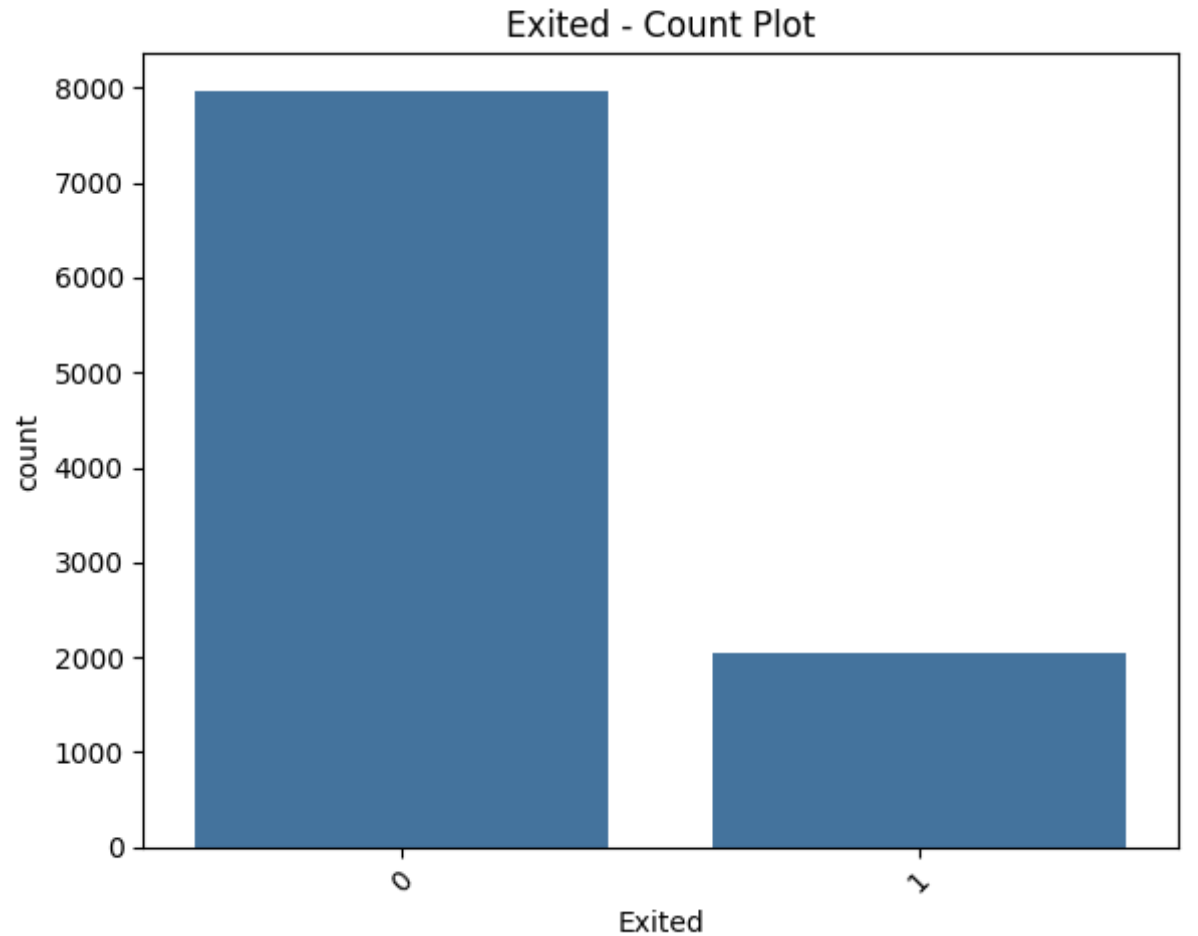
\includegraphics[width=\linewidth]{figures/churn_distribution.png}

\column{0.4\textwidth}

\begin{block}{Observation}
\begin{itemize}
    \item Approximately 20\% of customers churned
    \item Dataset is moderately imbalanced
    \item Evaluation focused on PR-AUC
    \item Class weighting applied in XGBoost
\end{itemize}
\end{block}

\end{columns}

\end{frame}

% ---------------- 7.1 EDA FINDINGS ----------------
\begin{frame}{EDA: Customer Complaints and Churn}

\begin{center}
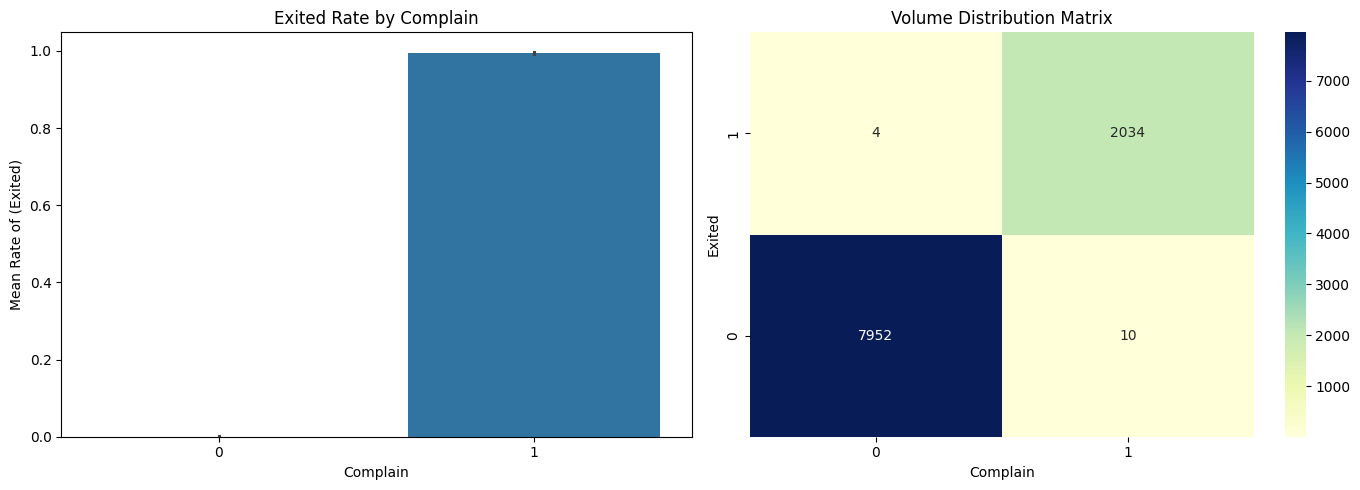
\includegraphics[width=0.75\linewidth]{figures/complain_churn.png}
\end{center}

\begin{alertblock}{Key Finding}
Customers who submitted complaints are substantially more likely to churn.
\end{alertblock}

\begin{itemize}
    \item Complaint status shows one of the strongest associations with churn.
    \item Customer service interactions appear to be a critical retention factor.
    \item The distribution suggests a strong positive correlation between complaints and churn.
\end{itemize}

\end{frame}

% ---------------- 7.2 EDA FINDINGS ----------------
\begin{frame}{EDA: Number of Products and Churn}

\begin{center}
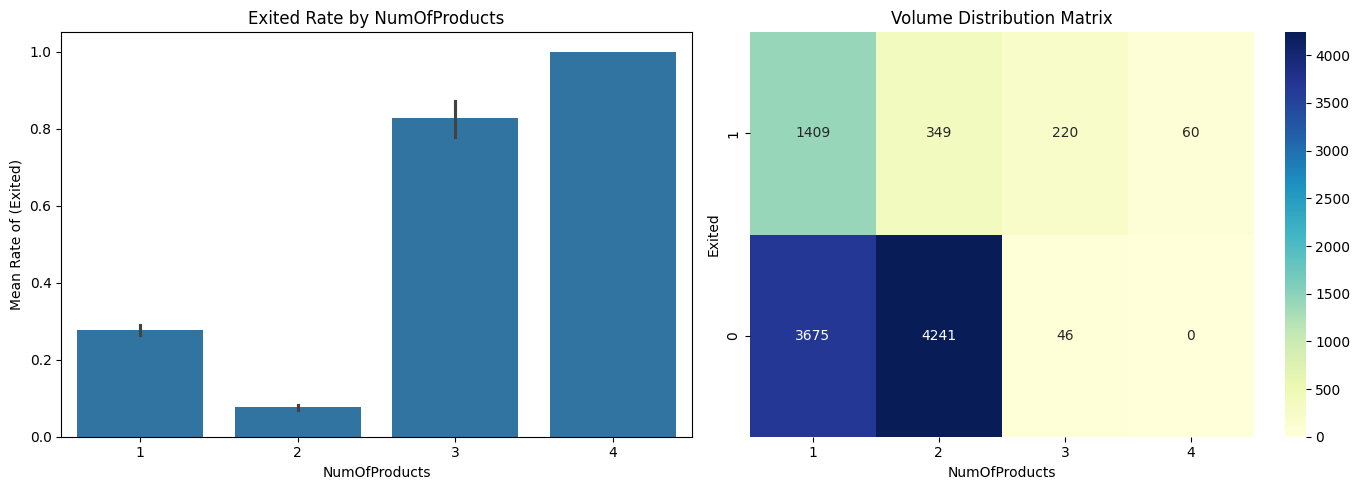
\includegraphics[width=0.75\linewidth]{figures/products_churn.png}
\end{center}

\begin{alertblock}{Key Finding}
Customers holding 3 or 4 products exhibit noticeably higher churn rates.
\end{alertblock}

\begin{itemize}
    \item Customers with 1--2 products are generally more stable.
    \item High-product customers may require targeted retention strategies.
\end{itemize}

\end{frame}

% ---------------- 7.3 EDA FINDINGS ----------------
\begin{frame}{EDA: Geography and Churn}

\begin{center}
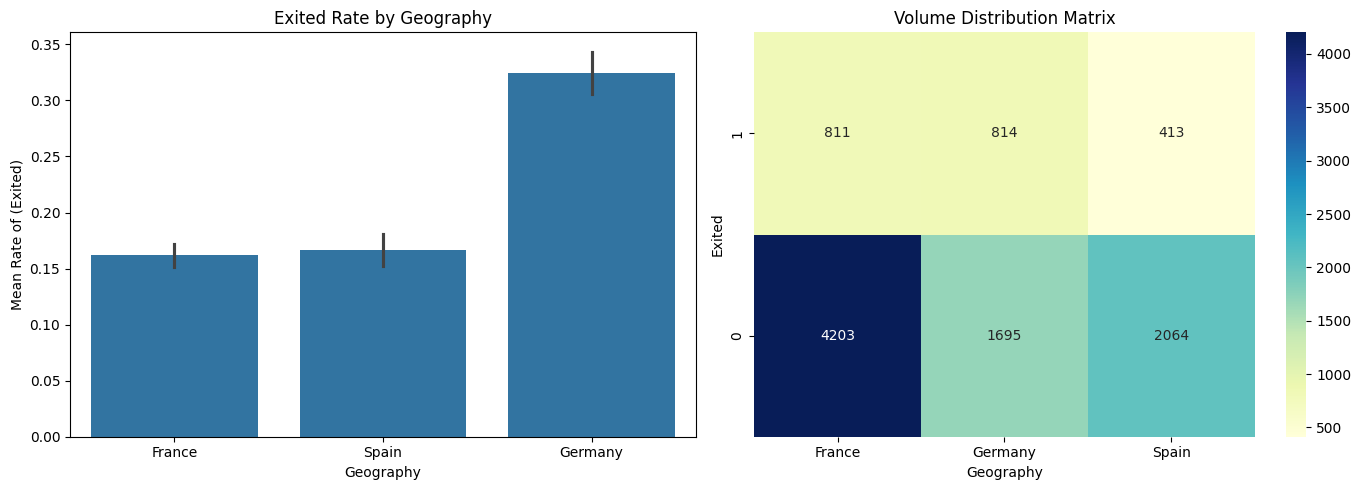
\includegraphics[width=0.75\linewidth]{figures/geography_churn.png}
\end{center}

\begin{alertblock}{Key Finding}
Customers in Germany exhibit significantly higher churn rates compared to France and Spain.
\end{alertblock}

\begin{itemize}
    \item Geographic location is a strong predictor of customer retention.
    \item Country-specific retention initiatives may be warranted.
\end{itemize}

\end{frame}

% ---------------- 7.4 EDA FINDINGS ----------------
\begin{frame}{EDA: Active Membership and Churn}

\begin{center}
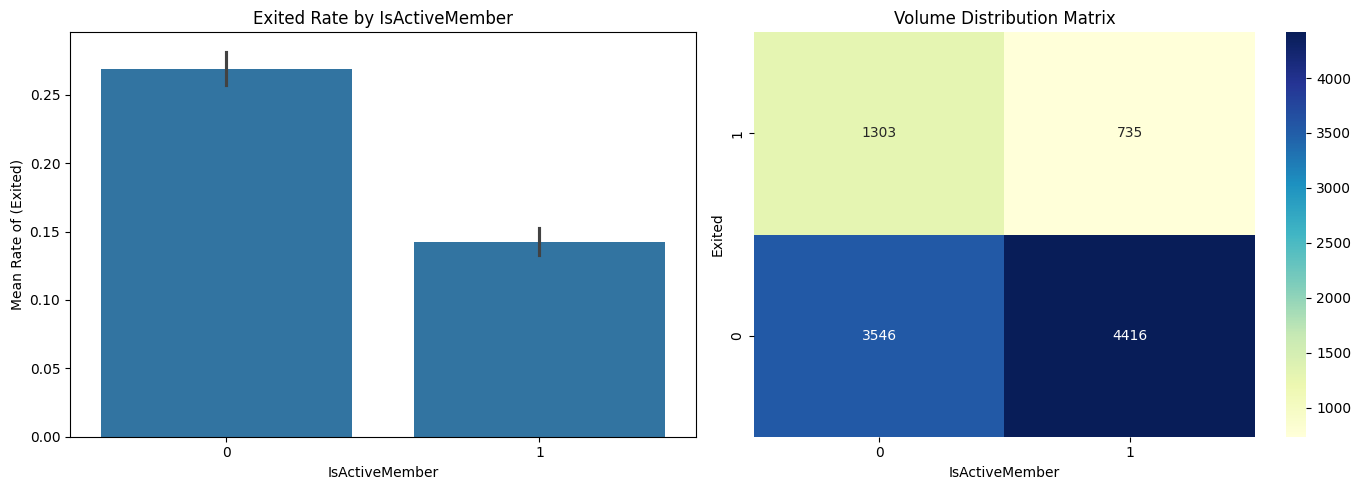
\includegraphics[width=0.75\linewidth]{figures/active_churn.png}
\end{center}

\begin{alertblock}{Key Finding}
Inactive customers churn at much higher rates than active members.
\end{alertblock}

\begin{itemize}
    \item Customer engagement strongly correlates with retention.
    \item Strategies to increase activity could reduce churn effectively.
\end{itemize}

\end{frame}

% ---------------- 8 DATA PREPROCESSING ----------------
\begin{frame}{Data Preparation}
\begin{itemize}
    \item No missing values detected; no imputation required.
    \item One-Hot Encoding applied to categorical features with \texttt{drop='first'} to avoid multicollinearity:
    \texttt{Card Type}, \texttt{NumOfProducts}, \texttt{Geography}, \texttt{Gender}.
    \item Standardization applied to continuous features:
    \texttt{Balance}, \texttt{Point Earned}, \texttt{CreditScore},
    \texttt{Age}, \texttt{Tenure}, \texttt{Satisfaction Score},
    \texttt{EstimatedSalary}.
    \item Binary features retained as-is:
    \texttt{HasCrCard}, \texttt{IsActiveMember}.
    \item Binary feature \texttt{Complain} was excluded from the analysis due to its strong correlation 
    with the target variable, which could introduce target leakage and artificially inflate model performance. 
    \item Train, validation, and test split performed after preprocessing.
\end{itemize}
\end{frame}

% ---------------- 9 BASELINE MODEL COMPARISON ----------------
\begin{frame}{Baseline Model Comparison}
\begin{itemize}
\item Several classification algorithms were evaluated using default hyperparameters:
\begin{itemize}
\item Logistic Regression
\item Decision Tree
\item Random Forest
\item XGBoost
\end{itemize}

\item Model performance was primarily assessed using Precision--Recall AUC (PR-AUC).

\item PR-AUC was preferred over Accuracy because customer churn prediction is an imbalanced classification problem.

\item In churn management, correctly identifying churners is more important than correctly classifying the majority non-churning customers.

\item Random Forest achieved the highest baseline PR-AUC (0.733), followed closely by XGBoost (0.692).

\end{itemize}
\end{frame}

% ---------------- 10 MODEL SELECTION ----------------
\begin{frame}{Model Selection for Optimization}
\begin{itemize}
\item Although Random Forest achieved the best performance with default settings, XGBoost was selected for further development.

\item The difference in baseline PR-AUC was relatively small (0.733 vs. 0.692).

\item XGBoost provides:
\begin{itemize}
    \item More extensive hyperparameter tuning capabilities.
    \item Gradient boosting optimization that often outperforms bagging methods after tuning.
    \item Built-in regularization to improve generalization.
    \item Better handling of complex feature interactions.
\end{itemize}

\item Therefore, XGBoost was considered the model with the highest potential for performance improvement during the modeling phase.

\end{itemize}
\end{frame}

% ---------------- 11 FEATURE IMPORTANCE ANALYSIS ----------------
\begin{frame}{Feature Importance Analysis}
    \footnotesize
\begin{itemize}
\item Feature importance was evaluated using the selected XGBoost model.

\item Customer product ownership was the strongest predictor of churn:
\begin{itemize}
    \item \texttt{NumOfProducts\_2} (25.8\%)
    \item \texttt{NumOfProducts\_3} (15.4\%)
    \item \texttt{NumOfProducts\_4} (8.4\%)
\end{itemize}

\item Customer engagement also showed high predictive power:
\begin{itemize}
    \item \texttt{IsActiveMember} (8.7\%)
    \item \texttt{Age} (6.6\%)
\end{itemize}

\item Geographic location contributed significantly:
\begin{itemize}
    \item \texttt{Geography\_Germany} (7.5\%)
    \item \texttt{Geography\_Spain} (2.7\%)
\end{itemize}

\item The five most important features represent approximately 66\% of the total feature importance assigned by the model.
\item Card type variables and credit card ownership contributed relatively little to churn prediction.

\end{itemize}
\end{frame}

% ---------------- 12 BUSINESS INSIGHTS ----------------
\begin{frame}{Key Business Insights}
\begin{itemize}
\item Product ownership is the primary driver of customer churn.

\item Active customers are substantially less likely to leave the bank.

\item Churn behavior varies across geographic regions, particularly in Germany.

\item Older customers exhibit different retention patterns than younger customers.

\item Credit card ownership and premium card tiers have limited impact on churn behavior.

\item Retention initiatives should prioritize:
\begin{enumerate}
    \item Customer engagement programs.
    \item Product portfolio optimization.
    \item Region-specific retention strategies.
\end{enumerate}

\end{itemize}
\end{frame}

% ---------------- 13 SHAP ANALYSIS ----------------
\begin{frame}{SHAP Model Interpretation}

\begin{columns}[T]

\begin{column}{0.55\textwidth}
\footnotesize
\begin{itemize}
    \item SHAP values were used to explain feature contributions to churn predictions.

    \item Factors increasing churn probability:
    \begin{itemize}
        \item Higher customer age
        \item Customers with 3 or 4 products
        \item German customers
        \item Higher account balances
    \end{itemize}

    \item Factors reducing churn probability:
    \begin{itemize}
        \item Active membership
        \item Customers with exactly 2 products
        \item Higher credit scores
    \end{itemize}
\end{itemize}
\end{column}

\begin{column}{0.45\textwidth}
\centering
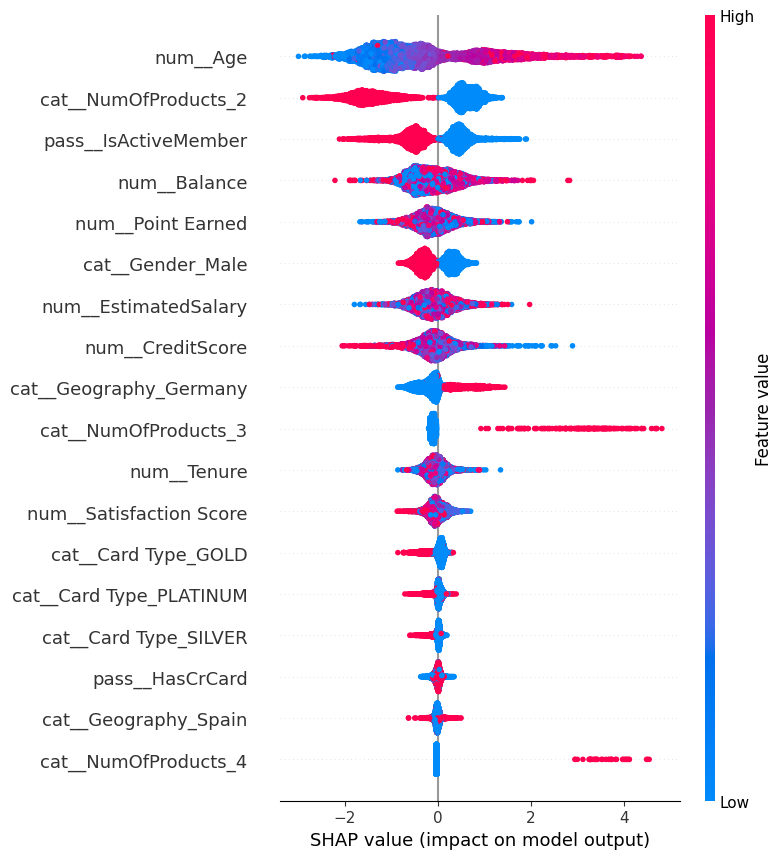
\includegraphics[width=\linewidth]{figures/shap_xgboost.png}

\vspace{0.2cm}
\tiny SHAP summary plot for the final XGBoost model.
\end{column}

\end{columns}

\end{frame}

% ---------------- 14 AGE EFFECT ANALYSIS: SHAP Dependence Plot ----------------
\begin{frame}{Age Effect on Churn Prediction: SHAP Dependence}

\begin{center}
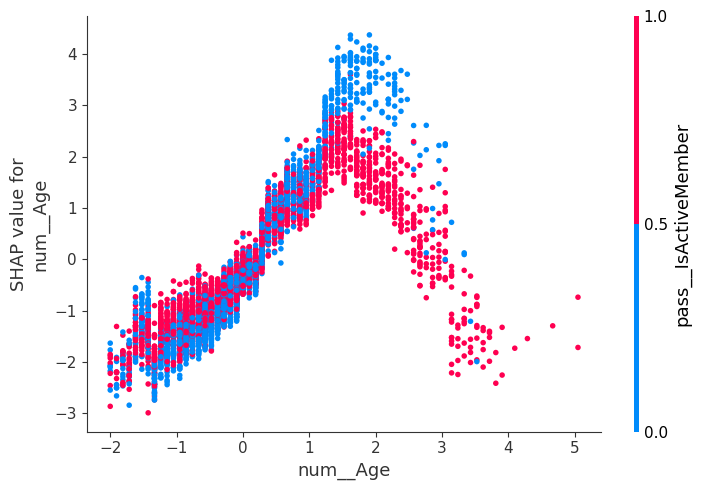
\includegraphics[width=0.75\textwidth]{figures/shap_dependence_num_age.png}

\vspace{0.3cm}
\tiny SHAP dependence plot for \texttt{Age}, colored by \texttt{IsActiveMember}.
\end{center}

\end{frame}

% ---------------- 15 AGE EFFECT ANALYSIS: Key Findings ----------------
\begin{frame}{Age Effect on Churn Prediction: Key Findings}

\footnotesize
\begin{itemize}
    \item Customer age exhibits a strong non-linear relationship with churn predictions.

    \item A transition occurs around standardized age $\approx 2.0$, where the SHAP contribution changes from positive to negative.

    \item Younger customers tend to significantly decrease the predicted probability of churn.

    \item Middle-age customers tend to increase the predicted probability of churn.

    \item Older customers tend to decrease the predicted probability of churn.

    \item Membership status moderates this effect:
    \begin{itemize}
        \item Inactive customers amplify the churn risk.
        \item Active customers further reduce the churn risk.
    \end{itemize}
\end{itemize}

\begin{block}{Business Insight}
Prioritize retention campaigns for middle-age customers, while older and younger customers represent a relatively low-risk segment.
\end{block}

\end{frame}

% ---------------- 16 FEATURE SELECTION RESULTS ----------------
\begin{frame}{Sequential Feature Selection Results}

\begin{block}{Methodology}
\scriptsize Sequential Feature Selection (Forward and Backward) was applied to Random Forest and XGBoost models, optimizing PR-AUC through 5-Fold Cross-Validation.
\end{block}

\begin{columns}[T]

\begin{column}{0.50\textwidth}

\scriptsize
\textbf{Best Configurations}
\begin{tabular}{lcc}
\hline
Model & Feat. & PR-AUC \\
\hline
\textbf{RF + Backward} & \textbf{17} & \textbf{0.6742} \\
XGB + Backward & 16 & 0.6688 \\
XGB + Forward & 12 & 0.6678 \\
RF + Forward & 27 & 0.6656 \\
\hline
\end{tabular}

\textbf{Observations}

\begin{itemize}
\scriptsize
\item Best overall result achieved by RF Backward SFS.
\item Peak performance reached with 17 selected features.
\item Backward elimination consistently outperformed forward selection.
\item Engineered interactions remained valuable even as feature count increased.
\end{itemize}

\end{column}

\begin{column}{0.50\textwidth}

\vspace{1cm}
\centering
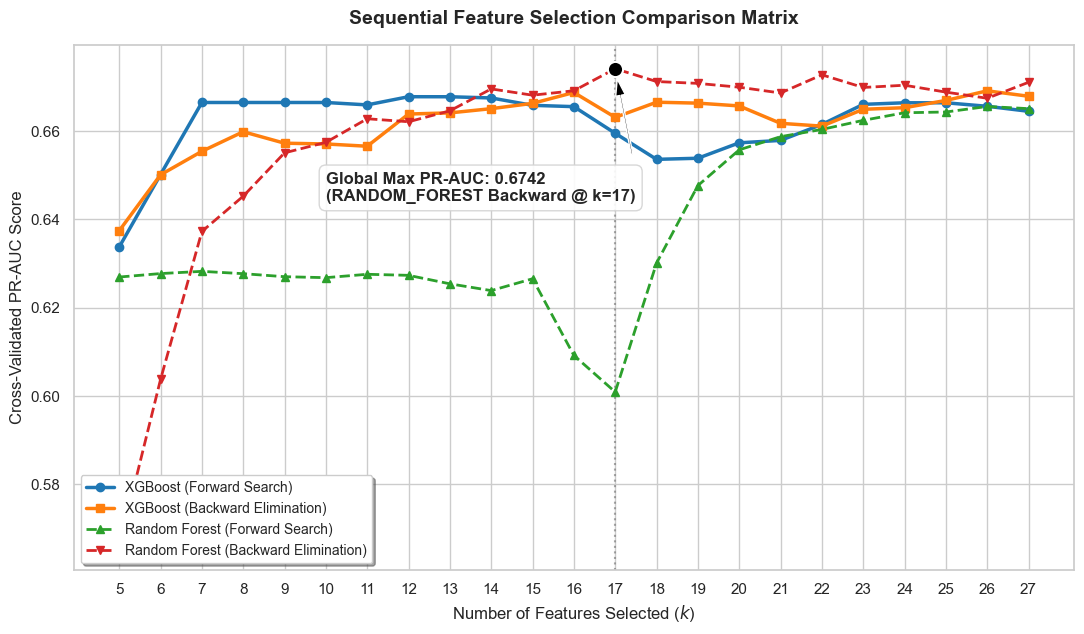
\includegraphics[width=\linewidth]
{figures/sequential_feature_selection.png}

\end{column}

\end{columns}

\end{frame}

% ---------------- 17 SELECTED FEATURES ----------------
\begin{frame}{Best Feature Subset Analysis}

\begin{block}{Winning Model}
\scriptsize
Random Forest with Backward Sequential Feature Selection achieved the highest
PR-AUC (\textbf{0.6742}) using a subset of \textbf{17 predictors}.
\end{block}

\scriptsize

\begin{columns}[T]

\begin{column}{0.45\textwidth}

\textbf{Selected Feature Groups}

\scriptsize
\begin{tabular}{p{1.7cm} p{3.3cm}}
\hline
\textbf{Category} & \textbf{Selected Features} \\
\hline
Demographics &
Gender, Germany, Spain \\

Products &
NumOfProducts\_1, 2, 3, 4 \\

Customer Value &
Estimated Salary, Point Earned, Satisfaction Score \\

Interactions &
Age$\times$IsActive,
CreditScore$\times$Age,
Inactive$\times$Balance \\

Ratios &
Balance per Product,
CreditScore per Age,
Products per Tenure \\

Card Type &
Silver Card \\
\hline
\end{tabular}

\end{column}

\begin{column}{0.55\textwidth}

\textbf{Key Findings}

\begin{itemize}
\footnotesize
\item Product ownership variables appeared in every high-performing subset.

\item Interaction features contributed more than raw customer attributes.

\item Financial ratios captured customer behavior better than standalone balance measures.

\item Geography remained a persistent source of churn heterogeneity.

\item Satisfaction and loyalty indicators added complementary predictive power.
\end{itemize}

\end{column}

\end{columns}

\end{frame}